% ##################################################################################################################
\section{Patna}
\label{sec:patna}
\hfill \textbf{Author:} Amit Agarwal

\editdone{This text has undergone the professional edit. Please no grammatical changes anymore! They are most-probably wrong.}

% ##################################################################################################################
Patna is a medium-size city in eastern India. As in other developing nations, traffic conditions are heterogeneous, composed of: a large number of bikes (37\,\%, including 4\,\% cycle rickshaws) and motorbikes (14\,\%). When this scenario was composed, public transport accounted for 18\,\% and walk for 29\,\%; only 2\,\% of all trips were made by car. Therefore, the \gls{matsim} queue simulation was modified to simulate travel demand under mixed traffic conditions.

A detailed Patna scenario description can be found in \citet[][]{AgarwalEtcMixedTraffic}. The scenario was created using household survey data from a comprehensive Patna mobility plan \citep[][]{TrippItransVks2009PatnaReport}, using the area within the Patna Municipal Corporation. The scenario consisted of 72\,zones, with a population of about 1.57\,million (year 2008). \gls{matsim} demand was generated using trip diaries, with car, motorbike and bike used as main congested modes (Figure~\ref{fig:patna0}). \gls{pcu} factors for different vehicle types were derived using effective area occupied by vehicles. The effective area occupied by a vehicle is calculated, and the ratio of area occupied by this vehicle to the area occupied by a passenger car is taken as \gls{pcu} factor for the respective vehicle.
%\karen{I am not clear what he means with "effective area occupied by vehicles"? Thanks.} 
To allow overtaking of slower vehicles (bike), by faster vehicles (car and motorbike), pre-existing, state-of-the-art \gls{fifo} queue simulation was overridden, using earliest link exit time as shown in Figure~\ref{fig:patna1}. Traffic behavior in modified queue simulation was then analyzed by plotting fundamental diagrams and space time trajectories for car, motorbike and bike.

%\ah{Could you please elaborate a little on computation time issue, \ie mention that there are none, if so.}
To address some special factors of Patna's travel time distributions, \gls{matsim} utility function was calibrated so that a mode share from real world data was replicated in the model, performed by allowing agents to switch modes. The model was validated using traffic count data and modal travel time distributions. The model's main shortcoming seemed to be overly short average travel times for motorbikes. Although no specific experiment was performed to analyze computational performance, no noticeable loss of performance was found during simulations. Thus, the model seems to be useful for many areas where mixed traffic conditions predominate.

\createfigure%
{Patna: Various vehicles on network, car in red, motorbike in blue and bike in green}%
{Patna: Various vehicles on network, car in red, motorbike in blue and bike in green}%
{\label{fig:patna0}}%
{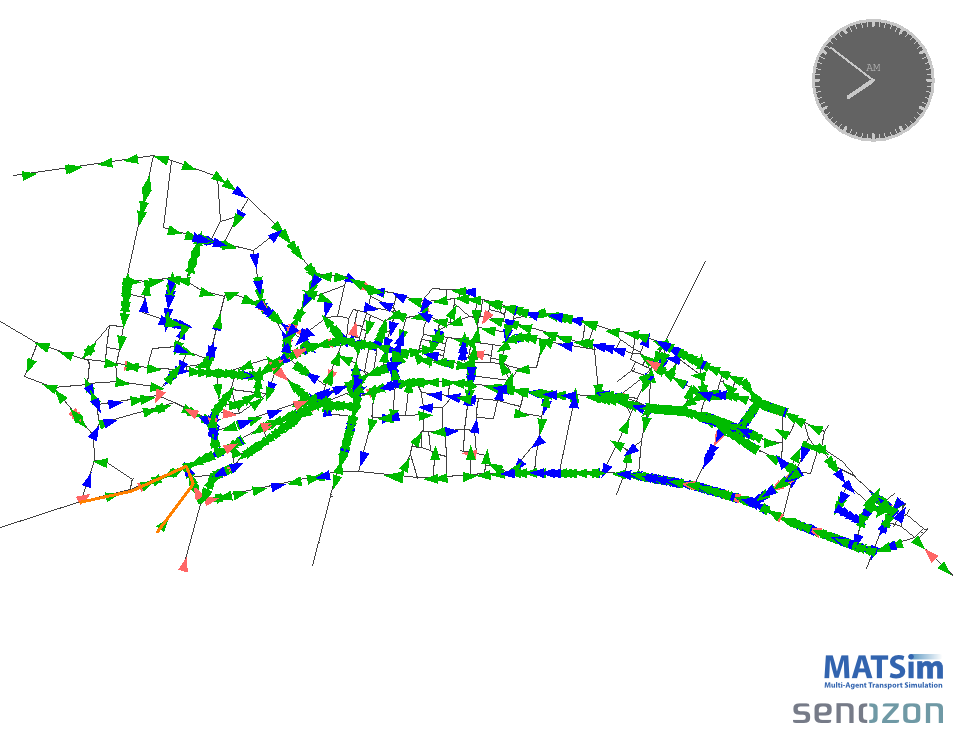
\includegraphics[width=0.99\textwidth, angle=0]{using/figures/vehiclesOnNetwork}}%
{}

\createfigure%
{Patna: \protect\gls{fifo} approach and passing of bicycle by car on a link (not to scale)}%
{Patna: \protect\gls{fifo} approach and passing of bicycle by car on a link (not to scale)}%
{\label{fig:patna1}}%
{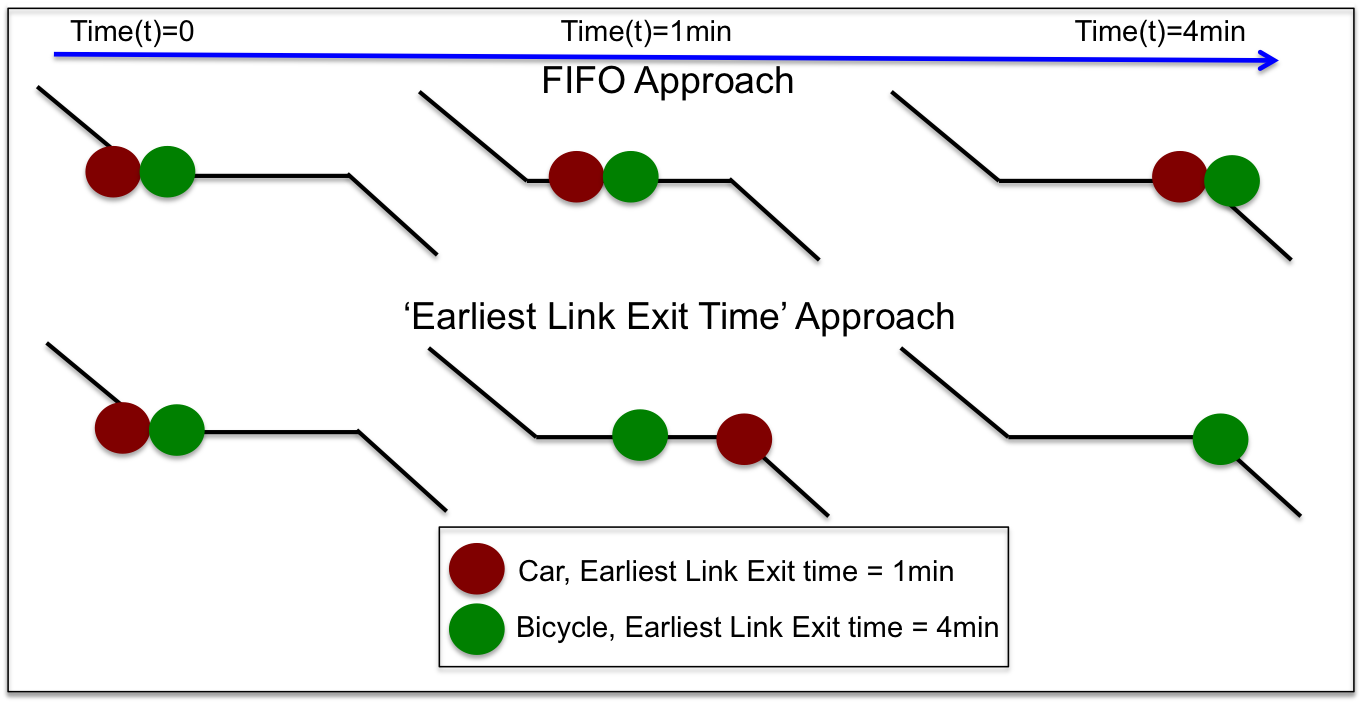
\includegraphics[width=0.99\textwidth, angle=0]{using/figures/FIFOandPassing}}%
{}

% ##################################################################################################################